\documentclass{article}
\usepackage{ctex}
\usepackage{ctex}  %使用宏包(为了能够显示汉字)
\title{基于规划和装箱模型的货物运输策略}  %文章标题
\author{周宇昕\quad 徐圣泽\quad 郑天宇}   %作者的名称
\date{\today}       %日期
\usepackage{amsmath}
\usepackage{amssymb}
\usepackage{multirow}
\usepackage{longtable}
\usepackage{graphicx}
\usepackage{subfigure}
\usepackage[a4paper,left=25mm,right=25mm,top=25mm,bottom=25mm]{geometry}  
\newcommand{\enabstractname}{Abstract}
\newcommand{\cnabstractname}{摘要}
\newenvironment{enabstract}{%
	\par\small
	\noindent\mbox{}\hfill{\bfseries \enabstractname}\hfill\mbox{}\par
	\vskip 2.5ex}{\par\vskip 2.5ex}
\newenvironment{cnabstract}{%
	\par\small
	\noindent\mbox{}\hfill{\bfseries \cnabstractname}\hfill\mbox{}\par
	\vskip 2.5ex}{\par\vskip 2.5ex}
\usepackage{listings}

\begin{document}
	\maketitle
	\begin{cnabstract}
	此次数学建模我们要解决是关于进出口公司货运飞机运输销售货物的装运策略问题。我们需要考虑装运飞机、装运货物等自身的限制,也要考虑最大经济效益,在不同特定情形下求解得到最优的策略和方案,以及对应的最大效益。

	第一个问题是求解特定情况下的最优装运方案。在本问中,我们采用规划模型,需要在满足约束条件的情况下,让飞机尽量不留空隙,即九个货舱中装入的货物占据尽可能大的空间,使得空间利用率尽可能高,因此目标函数便是关于最大容积利用率的函数。在相应质量、体积的约束条件下,即可求得三种飞机内的最佳装运策略。
	

	在第二个问题中,我们要解决两个问题。一个是集装箱的装载策略,另一个则是最终所有货物的装运策略,两者都是基于规划模型。目标函数仍是关于最大容积利用率的函数,约束条件需要在第一问基础上额外考虑集装箱的厚度、体积、自重以及对于集装箱和货物数量的限制。对于集装箱的装载策略,基于假设,我们引入装箱模型,利用规划约束,对各待装集装箱的货物选取空间利用率较大且各方面合适的“最优集装箱”。确定集装箱后,可得所有待运输货物,同样利用规划模型,以容积利用率为目标函数,可以得到三种飞机的装运策略。
	

	在第三问中,目标函数发生变化,变为关于最大利润的函数。在题目中未给出飞机的成本等费用,因此在本问题的解答过程中,我们对相关量进行人工定义。

	在第四和第五问中,通过观察数据,我们建立了相应的正态分布的概率统计模型,可以分别得到在可靠性为95\%和70\%时公司需要组织的各货品货源量。根据这些货物数量,代入前几问的模型中,可得到三种飞机的装运策略,并计算得到相应的最佳利润。
	
	至此,论文正文部分全部结束,在附录我们附上了算法实现的代码和其中部分运输方案的显式展现。
	
	\par\textbf{关键字:规划模型,目标函数,分支定界算法,装箱算法,正态分布} 
	\end{cnabstract}
	
	\newpage
	\section{情景概述}
	进出口公司经常需要将销售的货物通过货运飞机进行运输。在此问题中,货运飞机有三种类型,每种飞机均有三种货舱,每个货舱有最大容积、最大载重量的限制。需要进行运输和销售的货物共有十种,每种货物的规格和单价等基本参数已知,货物可以在一个或多个货舱中任意分布,多种货物可以混装。本题需要在三个货舱实际载重与最大载重尽可能成比例的情况下,满足不同场景下的不同要求,根据题目要求建立数学模型,求出相应的装运方案与最佳利润。
	
	\section{解决思路}
	\subsection{基本假设}
	\begin{itemize}
		\item[(1)]为简化问题,规定每一种集装箱内只装一种货物。
		\item[(2)]集装箱内的货物摆放时不倾倒,高度与附表中高度保持一致,即货物底面与集装箱底面平行。
		\item[(3)]集装箱的数量限制为每架次飞机运输时的数量限制。
		\item[(4)]考虑利润时只考虑货物成本、货物运输成本、飞行飞行成本,其余成本不予考虑。
	\end{itemize}
	
	\subsection{解决方向}
	该问题为规划问题的一种,我们采用规划的方法。规划问题由约束条件和目标函数组成,由题设,每个小问的场景都分别需要满足不同的约束条件,目标函数也各有不同。
	
	在实际的情况中,有些约束条件必须满足,如装箱问题中尺寸和质量等条件,但也会存在一些约束条件无法严格满足,例如本问题中所提到的“货舱中实际载重与最大载重成比例”,因此这些约束条件我们将之视为软约束,在实现的过程中只需要在一定的范围内成比例即可。
	
	除此之外,本题的目标函数其相关影响因素还有很多,如果仅仅考虑题目中给出的条件和数据,无法权衡并得到最优的目标函数。同时各个小题的目标函数也随场景发生变化,因此在解题的过程中,我们可能会人为定义一些条件,便于目标函数最优解的实现。	
	
	\section{变量声明及数据预处理}
	\subsection{变量声明}
	在解决本题的过程中,由于所设变量数较多,于是我们将多次用到的变量和符号名记录在下表中:
	\begin{table}[!h]
		\centering
		\caption{模型所需变量}
		\begin{tabular}{|l|l|}
			\hline
			变量 & 变量名 \\
			\hline
			舱体(集装箱)体积 & $V$\\
			舱体最大载重& $M$\\
			货物体积 &$v$\\
			货物重量 &$m$\\
			货物长 &$l$\\
			货物宽 &$w$\\
			货物高 &$h$\\
			舱中货物数量 &$a$\\
			货物供应数量 &$n$\\
			质量约束参数 &$s$\\
			飞机飞行成本 &$W$\\
			\hline
		\end{tabular}
	\end{table}

	\newpage
	\subsection{数据预处理}
	\begin{table}[!h]
		\centering
		\caption{飞机规格}
		\begin{tabular}{|c|c|c|c|c|c|c|}
			\hline
			舱体   & \multicolumn{2}{c|}{前舱} & \multicolumn{2}{c|}{中舱} & \multicolumn{2}{c|}{后舱} \\ \hline
			飞机参数 & 体积           & 最大载重     & 体积           & 最大载重     & 体积           & 最大载重     \\ \hline
			小型飞机 & 117.3        & 6        & 140.76       & 8        & 105.57       & 4        \\ \hline
			中型飞机 & 838.44       & 8        & 1321.776     & 12       & 691.028      & 6        \\ \hline
			大型飞机 & 2038.14      & 10       & 2501.2       & 16       & 1703.52      & 8        \\ \hline
		\end{tabular}
	\end{table}
	\begin{table}[!h]
		\centering
		\caption{货物规格}
		\begin{tabular}{|c|c|c|c|c|c|c|c|c|c|c|}
			\hline
			种类 & HW1   & HW2   & HW3  & HW4   & HW5   & HW6  & HW7   & HW8  & HW9  & HW10 \\ \hline
			体积 & 7.593 & 1.158 & 5.71 & 5.067 & 2.406 & 0.71 & 0.214 & 2.47 & 2.87 & 1.5  \\ \hline
			重量 & 2.1   & 0.2   & 0.7  & 1.8   & 1.3   & 0.3  & 0.23  & 1.2  & 0.9  & 0.3  \\ \hline
		\end{tabular}
	\end{table}
	\begin{table}[!h]
		\centering
		\caption{货物平均数量与利润}
		\begin{tabular}{|c|c|c|c|}
			\hline
			货物种类 & 单件利润 & 装运数量 & 利润      \\ \hline
			HW1  & 2000 & 119  & 238000  \\ \hline
			HW2  & 450  & 368  & 165600  \\ \hline
			HW3  & 2700 & 361  & 974700  \\ \hline
			HW4  & 2180 & 364  & 793520  \\ \hline
			HW5  & 1320 & 247  & 326040  \\ \hline
			HW6  & 440  & 307  & 135080  \\ \hline
			HW7  & 150  & 611  & 91650   \\ \hline
			HW8  & 1280 & 2993 & 3831040 \\ \hline
			HW9  & 1200 & 617  & 740400  \\ \hline
			HW10 & 700  & 1225 & 857500  \\ \hline
		\end{tabular}
	\end{table}

	\section{问题求解及结果}
	\subsection{第一问}
	第一问是针对三架飞机装运情况下容积利用率最大的货物装运方案。这个问题初看是一个复杂的三维装箱问题,但通过对数据的进一步分析,我们发现影响货物装运的主要是质量,其中体积的影响并不大,即在满足载重条件下的货物装运方案基本满足三维装箱的要求,所以我们可以把问题简化为一个规划问题。而又由题目所述,货物不必全部装完,所以我们可以仅考虑飞机运输一次的最佳策略。该条件下,货物的数量是足够的,也不用纳入考虑范围。三种飞机又是独立的,所以我们先以大飞机为例,建立我们的规划模型。
	
	如前分析所述,目标函数为飞机的容积利用率:
	\begin{equation}
		max\quad  K=\frac{\sum_{i=1}^{3}\sum_{j=1}^{10}a_{ij}v_{j}}{\sum_{i=1}^{3}V_{i}}
	\end{equation}
	其中,$i=1,2,3$分别指代一个飞机的前、中、后舱,$V_{i}$即代表相应舱的体积,$j$代表货物的类型,$v_{j}$是第$j$种货物的体积,$a_{ij}$即代表在$i$舱内第$j$种货物的数量,为整数。
	
	约束条件一:每个货舱中的货物总体积不超过货舱的最大容积。
	\begin{equation}
		\sum_{j=1}^{10}a_{ij}v_{j}\leq V_{i},\quad i=1,2,3
	\end{equation}
	
	约束条件二:每个货舱中的货物总质量不超过货舱的最大载重。
	\begin{equation}
		\sum_{j=1}^{10}a_{ij}m_{j}\leq M_{i},\quad i=1,2,3
	\end{equation}
	
	其中,$M_{i}$即代表相应舱的最大载重,$m_{j}$是第$j$种货物的质量。
	
	约束条件三:为了保证飞机飞行平稳,每个飞机三个货舱中实际载重必须与其最大载重成比例。考虑到实际情况,实际载重与最大载重很难实现严格成比例,因此我们可以人为适当放宽约束条件,引入质量比例约束的参数$s$,将本约束条件视为一个软约束,即允许在一定的范围内成比例。式子的具体表现形式如下:
	\begin{equation}
		\left|\frac{\sum_{j=1}^{10}a_{1,j}m_{j}}{M_{1}}-\frac{\sum_{j=1}^{10}a_{2,j}m_{j}}{M_{2}}\right|<s
	\end{equation}
	\begin{equation}
		\left|\frac{\sum_{j=1}^{10}a_{1,j}m_{j}}{M_{1}}-\frac{\sum_{j=1}^{10}a_{3,j}m_{j}}{M_{3}}\right|<s
	\end{equation}
	\begin{equation}
		\left|\frac{\sum_{j=1}^{10}a_{2,j}m_{j}}{M_{2}}-\frac{\sum_{j=1}^{10}a_{3,j}m_{j}}{M_{3}}\right|<s
	\end{equation}
	在本文之后的规划中,无特殊情况,我们统一取$s=0.1$,认为在该约束下,基本实现了货舱中实际载重与最大载重成比例。
	
	于是基于以上规划模型,我们用lingo软件编写相应程序,最终可以得到各飞机各舱内的装载结果,如下表和图所示:
	\newpage
	\begin{table}[!h]
		\centering
		\caption{装运方法}
		\begin{tabular}{|c|c|c|c|}
			\hline
			& 小型飞机             & 中型飞机         & 大型飞机         \\ \hline
			前舱 & 2号2个 3号8个       & 3号11个 10号1个 & 2号1个 3号14个  \\ \hline
			中舱 & 3号11个 10号1个     & 3号17个       & 2号3个 3号22个  \\ \hline
			后舱 & 2号1个 3号5个 10号1个 & 2号2个 3号8个   & 3号11个 10号1个 \\ \hline
			容积率 & $39.5\%$ & $7.35\%$ & $4.40\%$  \\ \hline
		\end{tabular}
	\end{table}

	\begin{figure}[!h]
		\centering 
		\subfigure[小飞机前舱]{
			\label{Fig.sub.1}
			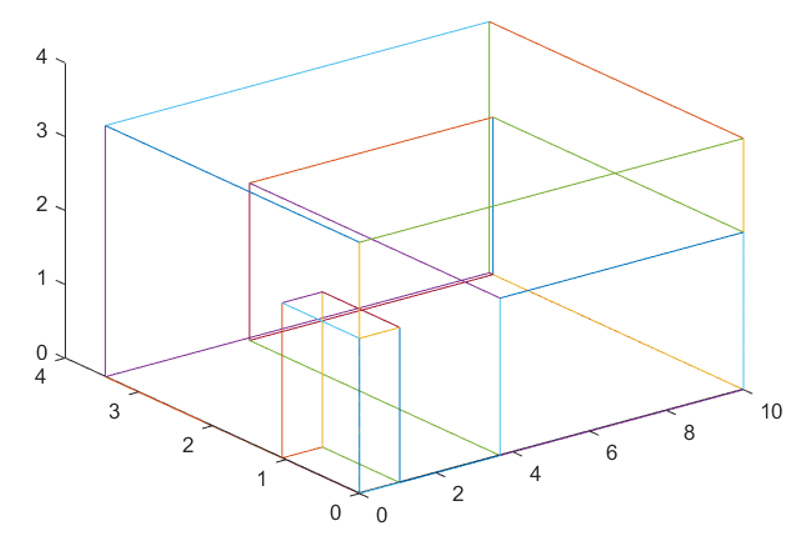
\includegraphics[width=0.4\textwidth]{小飞机前舱.png}}
		\subfigure[小飞机中舱]{
			\label{Fig.sub.2}
			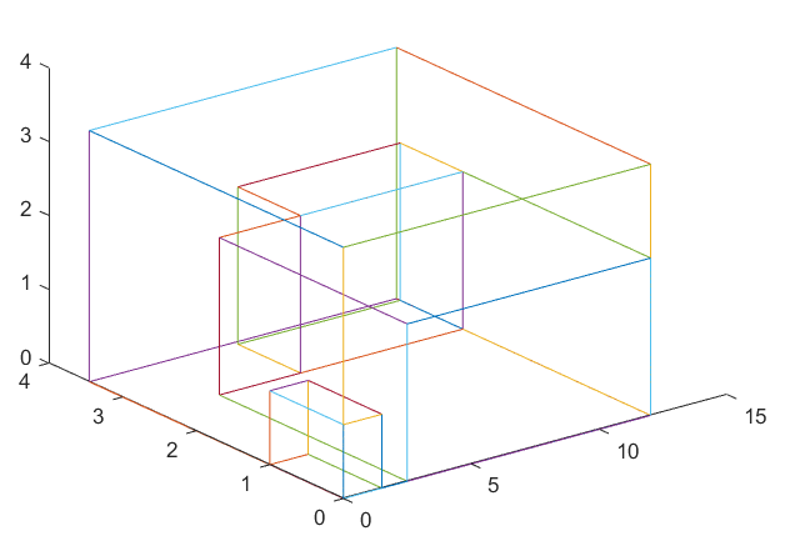
\includegraphics[width=0.4\textwidth]{小飞机中舱.png}}
		\subfigure[小飞机后舱]{
			\label{Fig.sub.3}
			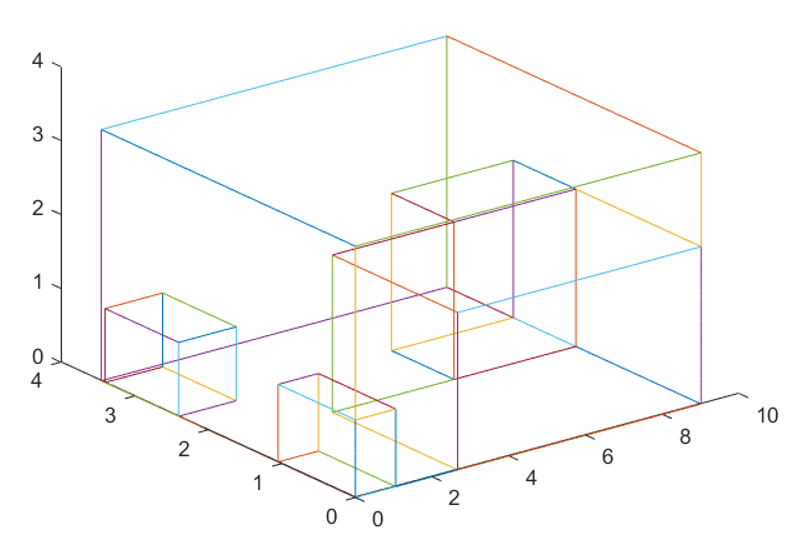
\includegraphics[width=0.4\textwidth]{小飞机后舱.png}}
	\end{figure}

	\newpage
	\begin{figure}[!h]
		\centering 
		\subfigure[中飞机前舱]{
			\label{Fig.sub.1}
			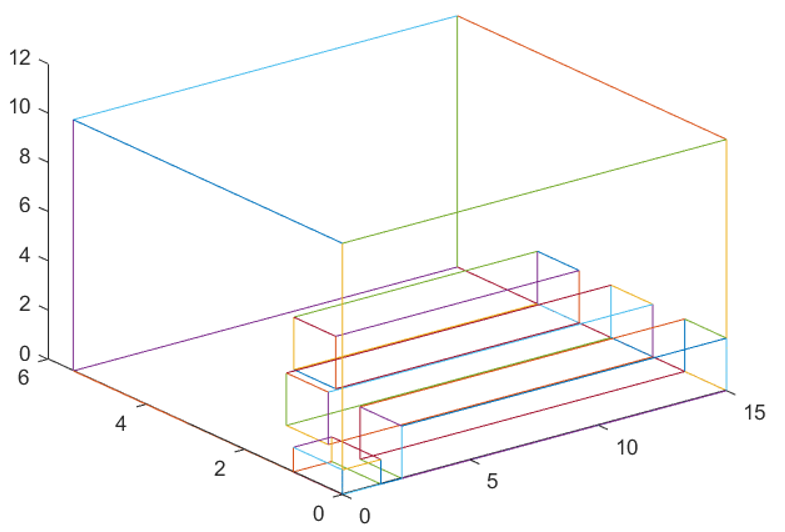
\includegraphics[width=0.4\textwidth]{中飞机前舱.png}}
		\subfigure[中飞机中舱]{
			\label{Fig.sub.2}
			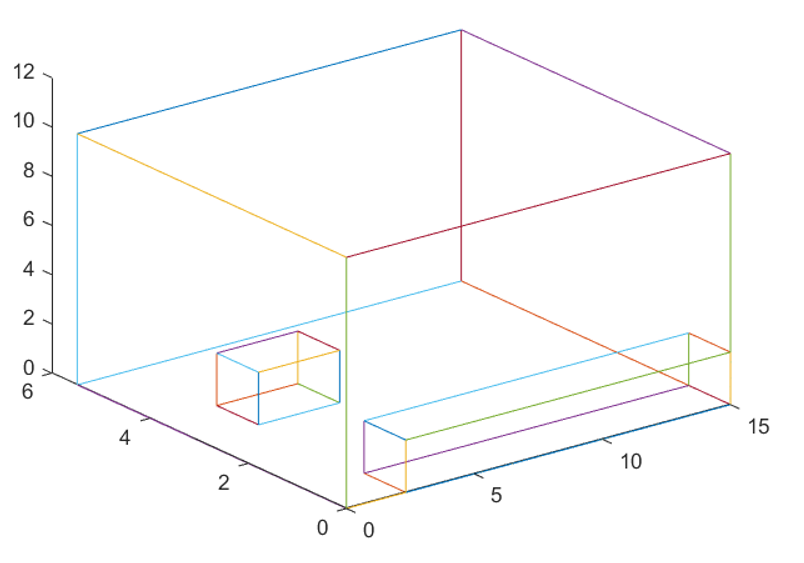
\includegraphics[width=0.4\textwidth]{中飞机中舱.png}}
		\subfigure[中飞机后舱]{
			\label{Fig.sub.3}
			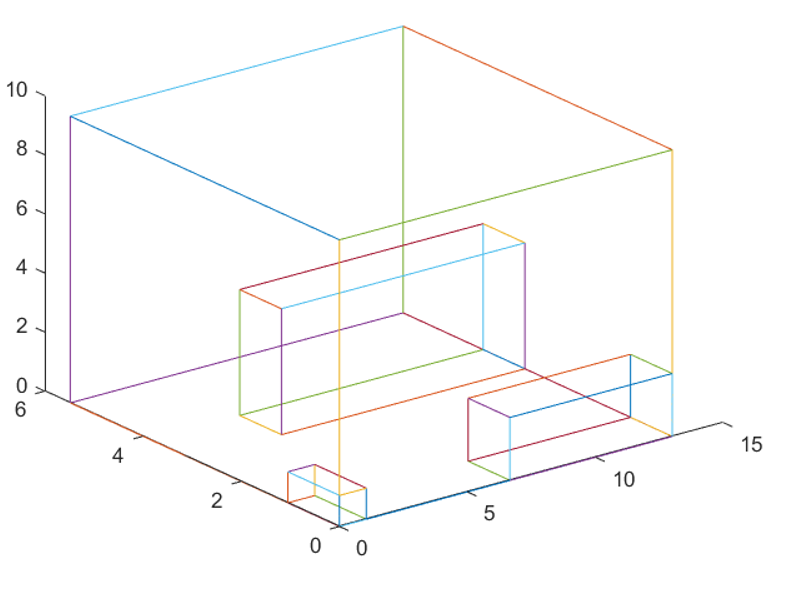
\includegraphics[width=0.4\textwidth]{中飞机后舱.png}}
	\end{figure}

	\begin{figure}[!h]
		\centering 
		\subfigure[大飞机前舱]{
			\label{Fig.sub.1}
			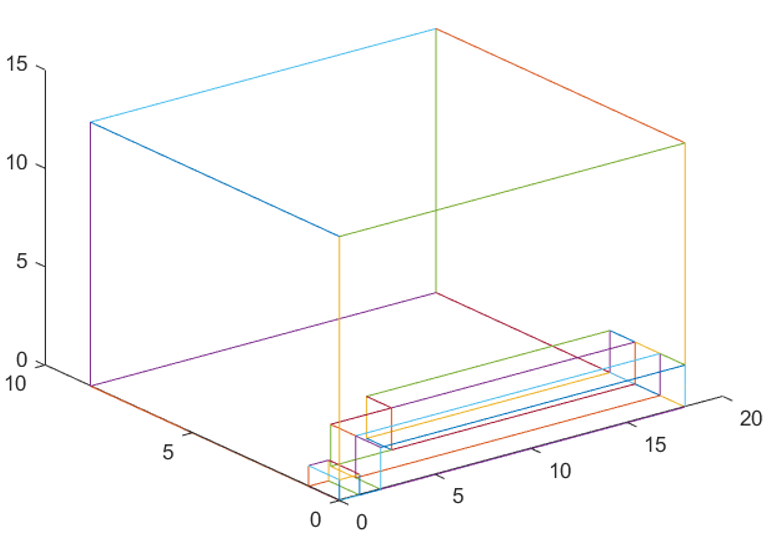
\includegraphics[width=0.4\textwidth]{大飞机前舱.png}}
		\subfigure[大飞机中舱]{
			\label{Fig.sub.2}
			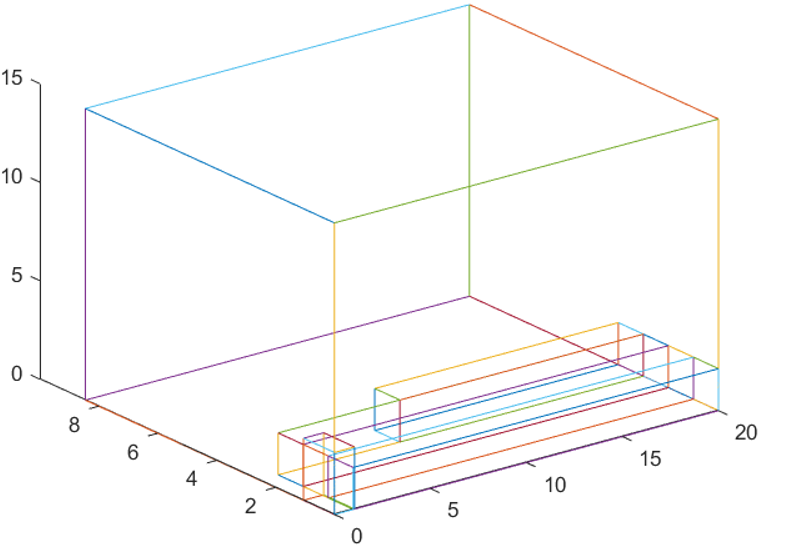
\includegraphics[width=0.4\textwidth]{大飞机中舱.png}}
		\subfigure[大飞机后舱]{
			\label{Fig.sub.3}
			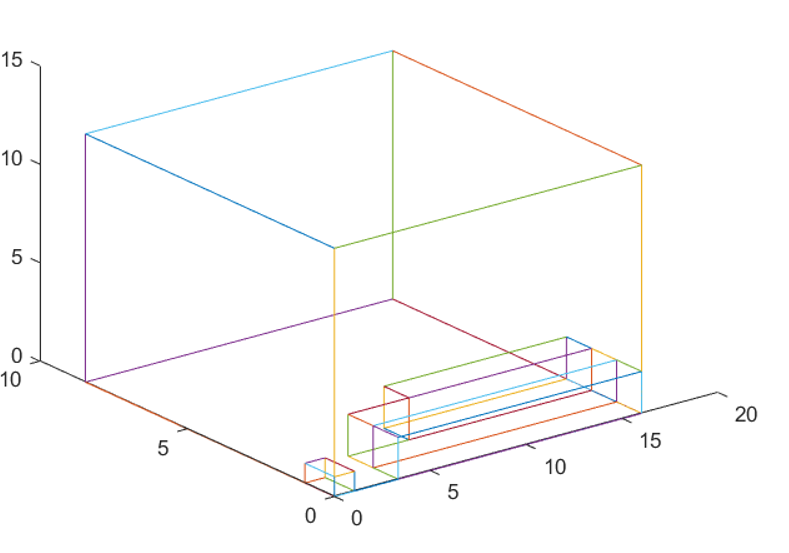
\includegraphics[width=0.4\textwidth]{大飞机后舱.png}}
	\end{figure}

	\newpage
	 \subsection{第二问}
	\subsubsection{集装箱装载策略}
	根据题目要求,体积在2$m^3$以下的货物都要用集装箱装载,即2、6、7、10四种货物要用集装箱装载,而对应的集装箱有7种。根据我们的假设,一种集装箱内只装一种货物,则对于每一种货物,我们要从这七种中选择最适合它的那种集装箱。由于要求为集装箱内尽量不留空隙,所以同样我们以容积率为参照指标,寻求容积率最大的装载策略。
	
	首先观察7种集装箱的数据,我们发现1、2、4、5号集装箱的体积规模是一样的,但是由于最后装入飞机时密度越小越有利,所以在这四种中我们应优先考虑质量最轻的4号,而其余3种不予考虑,所以最终待考察的集装箱对象为3、4、6、7四种。而将货物装入集装箱的问题是一个装箱问题。
	
	对于装箱问题,我们也可以将其视为一个规划。目标函数仍为容积率:
	\begin{equation}
		max\quad  K=\frac{\sum_{j=1}^{n_i}l_{ij}w_{ij}h_{ij}}{V_{i}}
	\end{equation}
	其中,$l_{ij}$、$w_{ij}$、$h_{ij}$为放入第$i$种集装箱中第$j$个货物的长、宽、高,$V_i$为第$i$种集装箱的容积,$n_i$为其中的货物数量。基本约束即为体积约束:
	\begin{equation}
		\sum_{j=1}^{n_i}l_{ij}w_{ij}h_{ij}\leq V_{i}
	\end{equation}
	由于我们假设货物放入集装箱时不能倾倒,即高保持不变,则该装箱问题实际上是一个二维装箱问题,求解它的具体思路如下:

	设导出装箱方法的函数为$N(x,g)$,自变量$x$表示填充物,$g$为被填充物,返回值是使得装箱数量最多的装箱方法。
	
	设变量$x$三边长度设为$ae$、$be$、$he$,变量$g$三边长度设为$ac$、$bc$、$hc$。
	\begin{figure}[!h]
		\centering 
		\subfigure[填充物尺寸]{
			\label{Fig.sub.1}
			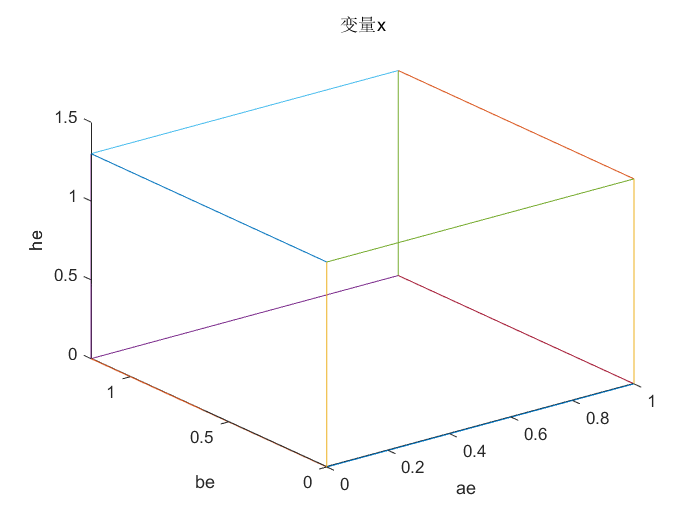
\includegraphics[width=0.4\textwidth]{填充物.png}}
		\subfigure[被填充物尺寸]{
			\label{Fig.sub.2}
			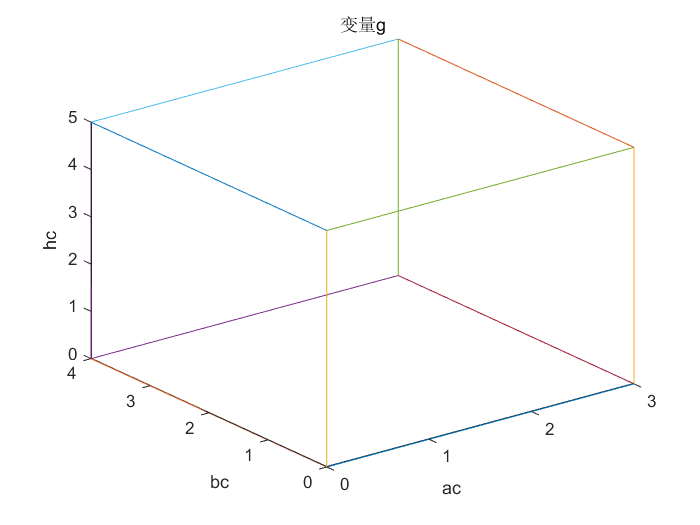
\includegraphics[width=0.4\textwidth]{被填充物.png}}
	\end{figure}

	首先明确最优装箱一定是填充物与被填充物的边平行,对于本题考虑现实情况在为了方便拿取搬运,$h$方向的装载方式固定,即$he$与$hc$始终平行,于是$N$变成了二维填充问题。
	
	填充从边角开始,对于第一块填充,$ae$和$be$与$ac$和$bc$的平行方式有两种:竖放和横放。
	
	若竖放,则$ae$平行$ac$、$be$平行$bc$,放置后对底面可以进行切割,共有两种切割方法。
	\begin{figure}[!h]
		\centering 
		\subfigure[方法1]{
			\label{Fig.sub.1}
			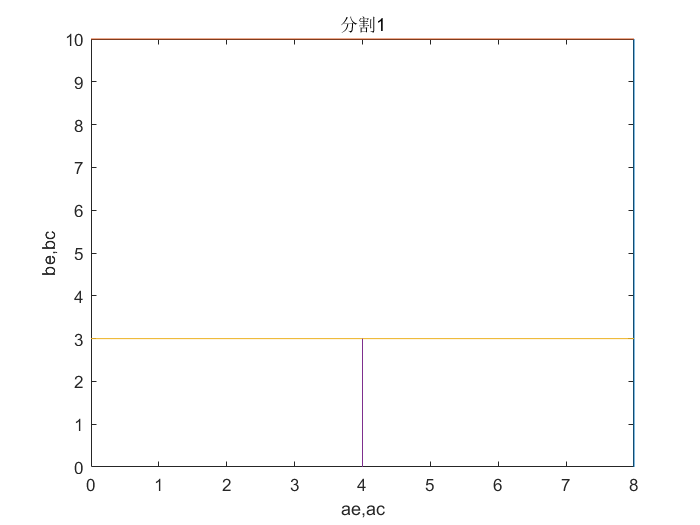
\includegraphics[width=0.4\textwidth]{分割1.png}}
		\subfigure[方法2]{
			\label{Fig.sub.2}
			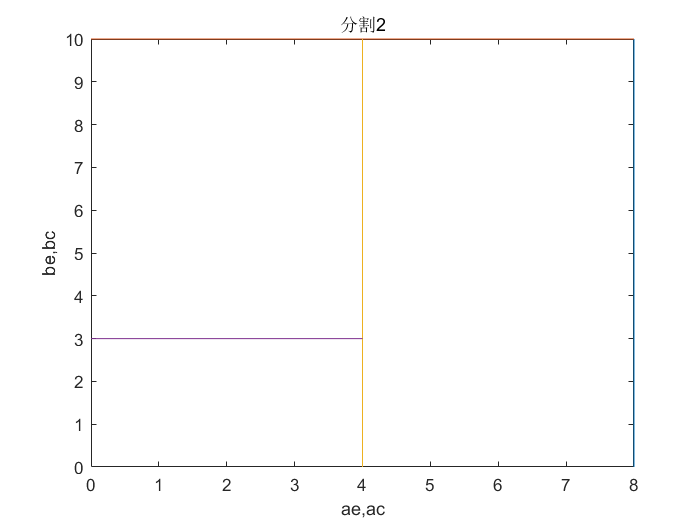
\includegraphics[width=0.4\textwidth]{分割2.png}}
	\end{figure}

	上下左右切出的四块分别为$g1$、$g2$、$g3$、$g4$,设竖放是最多填充方式函数为$N1(x,g)$,有$N1(x,g)=Max((Upright+N1(g1,x)+N1(g2,x)),(Upright+N1(g3,x)+N1(g4,x)))$,$_Max$表示填充数多的方法。同理写出$N2$,有$N=max(N1,N2)$。
	
	于是本题转化为一个迭代问题,迭代达到终点的标志为:当($ae>ac$且$ae>bc$)或($be>ac$且$be>bc$)或($ae>ac$且$be>ac$)或($ae>bc$且$be>bc$)时。
	
	接下来我们进行一些操作来简化装箱问题。当填充物与被填充物体积相差不多、一般数量级小于一百时,可以发现最优装箱有一定的规律,此时可以按下面步骤装箱。
	
	首先取$ac$或$bc$为竖方向,若取$ac$为竖方向,此时$bc$方向上货物取为同向,即一排上同向,一列上呈现横竖分布,设横竖分别$x$和$y$个,此时$x>=0$,$y>=0$,$ae*x+be*y<=bc$,情况可穷尽。同理$bc$为竖直也可穷尽,可以取装箱量最多的情况。
	

	\begin{table}[!h]
		\centering
		\caption{货物与集装箱}
		\begin{tabular}{|c|c|c|c|c|c|c|c|c|c|c|}
			\hline
			\multirow{2}{*}{} & \multicolumn{2}{c|}{3号箱} & \multicolumn{2}{c|}{4号箱} & \multicolumn{3}{c|}{6号箱}                  & \multicolumn{3}{c|}{7号箱}                  \\ \cline{2-11} 
			& 数量       & 容积率         & 数量       & 容积率         & 数量 & 容积率    & \multicolumn{1}{l|}{放置高度} & 数量 & 容积率    & \multicolumn{1}{l|}{放置高度} \\ \hline
			货物2               & 2          & 40.6\%      & 8          & 58.6\%      & 2    & 69.3\% & 1.05                      & 4    & 78.2\% & 1.05                      \\ \hline
			货物6               & 6          & 74.6\%      & 12         & 53.9\%      & 6    & 79.7\% & 1.68                      & 12   & 89.8\% & 1.68                      \\ \hline
			货物7               & 18         & 67.5\%      & 56         & 75.8\%      & 18   & 77.7\% & 1.56                      & 36   & 87.5\% & 1.56                      \\ \hline
			货物10              & 1          & 26.3\%      & 6          & 57.0\%      & 1    & 47.2\% & 1                         & 6    & 79.7\% & 2                         \\ \hline
		\end{tabular}
	\end{table}

	以上是根据装箱算法得出的比较结果。由表中结果可知,四种货物放入7号集装箱都是容积率最大的最优选择。但是计算它们的质量时我们发现一个问题,即7号货物装入7号集装箱质量达$8.43t$,这严重超过了小飞机的载重,这种情况应当避免。所以,退而求其次,我们选择将7号货物装入6号集装箱,最终这四种货物放入集装箱的示意图如下:
	\begin{figure}[!h]
		\centering 
		\subfigure[货物2装入7号集装箱]{
			\label{Fig.sub.1}
			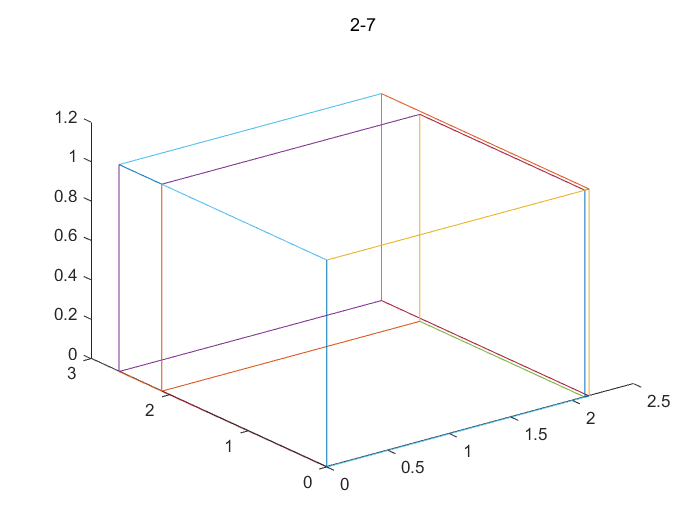
\includegraphics[width=0.4\textwidth]{2-7.png}}
		\subfigure[货物6装入7号集装箱]{
			\label{Fig.sub.2}
			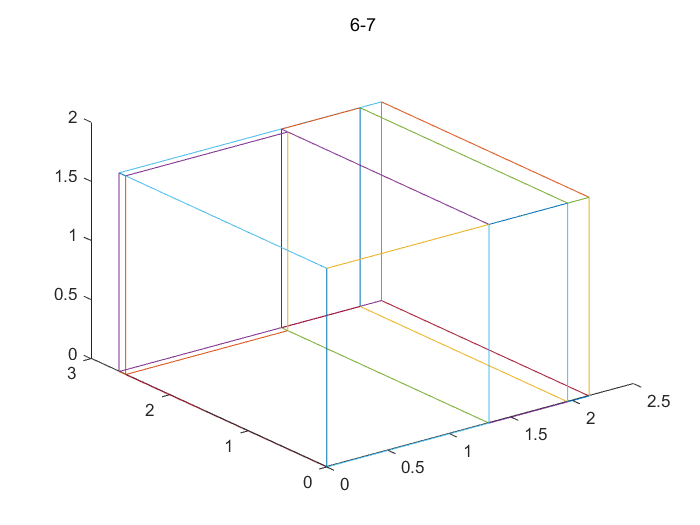
\includegraphics[width=0.4\textwidth]{6-7.png}}
		\subfigure[货物7装入6号集装箱]{
			\label{Fig.sub.3}
			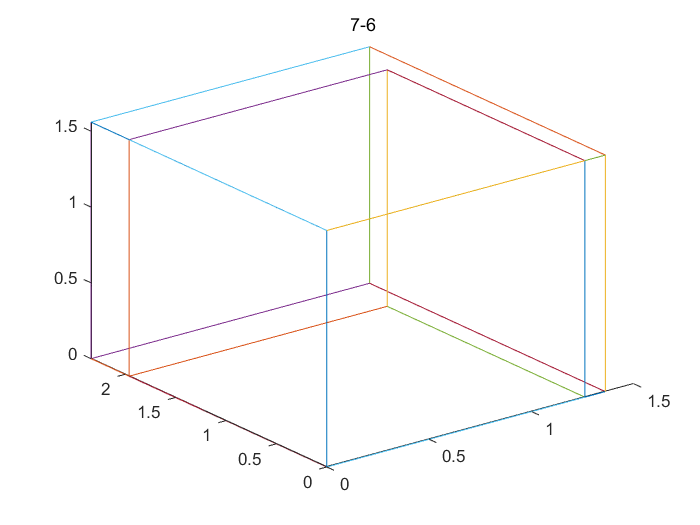
\includegraphics[width=0.4\textwidth]{7-6.png}}
		\subfigure[货物10装入7号集装箱]{
			\label{Fig.sub.4}
			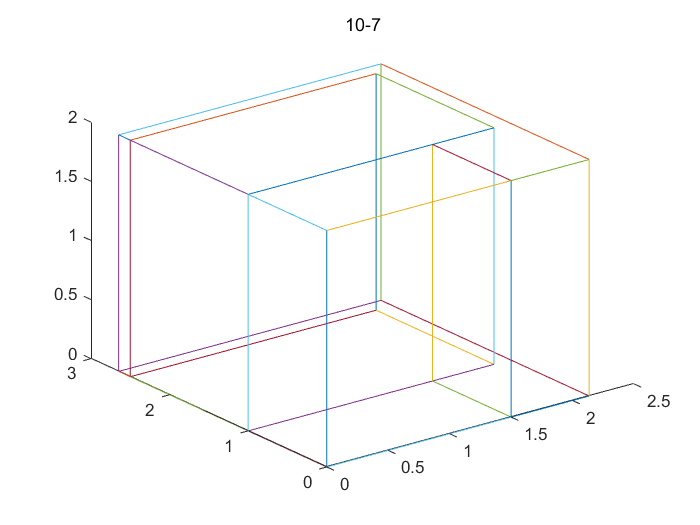
\includegraphics[width=0.4\textwidth]{10-7.png}}
	\end{figure}
	
	\newpage
	\subsubsection{货物装运策略}
	在第二问中,我们要按照前50个周期各种货物销售量的平均值组织货源。基于前面集装箱的讨论分析,我们可以把原先的2、6、7、10四种货物装入它们对应的集装箱,得到有新质量和体积的2、6、7、10号集装箱,之后仍以2、6、7、10号货物称代。新的2、6、7、10号货物的数量为92,26,34和205个。接着在考虑装运时,我们以每一次的最优解为考虑方案,与第1问类似,同样可以建立规划模型,其目标和约束均类似。只不过此时我们要将货物运送完,在货物数量上会随着优化求解的一步步进行而减少,为此我们引入货物数量$n_{j}$,$j$为货物种类,约束条件为
	\begin{equation}
		\sum_{i=1}^{3}a_{ij}\leq n_j ,\quad j=1,2,\cdots,10
	\end{equation}
	此外,由于6、7号集装箱有数量限制,都至多为10个,所以还要加上关于集装箱数量的条件约束:
	\begin{equation}
		a_{1,2}+a_{2,2}+a_{3,2}+a_{1,6}+a_{2,6}+a_{3,6}+a_{1,10}+a_{2,10}+a_{3,10}\leq 10;
	\end{equation}
	\begin{equation}
		a_{1,7}+a_{2,7}+a_{3,7}\leq 10;
	\end{equation}
	至此,根据这些约束条件,我们可以用lingo求解相应的装运策略,在过程中不断调整货物数量,最终可得三种飞机下不同的装运方案如下:
	\newpage
	\begin{table}[!h]
		\centering
		\caption{小飞机装运方案}
		\begin{tabular}{|c|c|c|c|c|c|}
			\hline
			小飞机方案 & 前舱        & 中舱         & 后舱                                                         & 总容积率   & 趟次  \\ \hline
			1     & 2号1个 3号7个 & 3号1个 3号10个 & 2号2个 3号3个                                                  & 0.392  & 18  \\ \hline
			2     & 10号3个     & 2号2个 10号3个 & 10号2个                                                      & 0.322  & 10  \\ \hline
			3     & 10号3个     & 10号4个      & 10号2个                                                      & 0.319  & 13  \\ \hline
			4     & 10号3个     & 10号4个      & \begin{tabular}[c]{@{}c@{}}3号1个 9号1个 \\ 10号1个\end{tabular} & 0.307  & 1   \\ \hline
			5     & 1号2个 9号2个 & 1号2个 9号4个  & 1号1个 9号2个                                                  & 0.168  & 23  \\ \hline
			6     & 1号2个 9号2个 & 1号2个 9号4个  & 9号4个                                                       & 0.162  & 1   \\ \hline
			7     & 9号6个      & 9号8个       & 9号4个                                                       & 0.142  & 23  \\ \hline
			8     & 6号1个 9号2个 & 6号2个       & 9号4个                                                       & 0.137  & 1   \\ \hline
			9     & 6号1个 9号2个 & 6号2个       & 6号1个                                                       & 0.136  & 1   \\ \hline
			10    & 4号1个 6号1个 & 6号2个       & 6号1个                                                       & 0.134  & 4   \\ \hline
			11    & 4号1个 6号1个 & 4号2个 6号1个  & 6号1个                                                       & 0.132  & 1   \\ \hline
			12    & 4号3个      & 4号4个       & 4号2个                                                       & 0.125  & 39  \\ \hline
			13    & 4号2个 8号2个 & 4号3个 8号2个  & 4号1个 8号1个                                                  & 0.118  & 1   \\ \hline
			14    & 8号5个      & 8号6个       & 8号3个                                                       & 0.091  & 213 \\ \hline
			15    & 8号5个      & 5号6个       & 5号2个 8号1个                                                  & 0.0937 & 1   \\ \hline
			16    & 5号4个      & 5号6个       & 5号3个                                                       & 0.086  & 18  \\ \hline
			17    & 5号1个 7号1个 & 5号2个 7号1个  & 5号2个                                                       & 0.0656 & 1   \\ \hline
			18    & 7号1个      & 7号1个       &                                                            & 0.0325 & 16  \\ \hline
		\end{tabular}
	\end{table}
	
	\newpage
	\begin{table}[!h]
		\centering
		\caption{中飞机装运方案}
		\begin{longtable}{|c|c|c|c|c|c|}
			\hline
			中飞机方案 & 前舱                                                              & 中舱                                                         & 后舱                                                              & 总容积率   & 趟次  \\ \hline
			1     & 2号1个 3号10个                                                      & 3号17个                                                      & 2号1个 3号7个                                                       & 7.31\% & 10  \\ \hline
			2     & 3号3个 10号3个                                                      & 2号6个 3号9个                                                  & 2号1个 3号7个                                                       & 6.89\% & 1   \\ \hline
			3     & 10号4个                                                           & \begin{tabular}[c]{@{}c@{}}3号2个 9号3个 \\ 10号4个\end{tabular} & 1号1个 10号2个                                                      & 5.48\% & 1   \\ \hline
			4     & 1号1个 10号3个                                                      & 1号1个 10号5个                                                 & 1号1个 10号2个                                                      & 5.31\% & 19  \\ \hline
			5     & \begin{tabular}[c]{@{}c@{}}1号2个 2号1个 \\ 9号1个 10号1个\end{tabular} & 1号3个 2号6个                                                  & \begin{tabular}[c]{@{}c@{}}1号1个 2号1个 \\ 9号1个 10号1个\end{tabular} & 4.68\% & 1   \\ \hline
			6     & 1号2个 2号4个                                                       & 1号3个 2号6个                                                  & 1号2个 9号2个                                                       & 4.54\% & 5   \\ \hline
			7     & 1号2个 2号4个                                                       & 1号4个 9号4个                                                  & \begin{tabular}[c]{@{}c@{}}1号1个 2号3个 \\ 9号1个\end{tabular}       & 4.10\% & 1   \\ \hline
			8     & 1号2个 9号4个                                                       & 1号4个 9号4个                                                  & 1号2个 9号2个                                                       & 3.14\% & 1   \\ \hline
			9     & 1号2个 9号4个                                                       & 1号1个 9号11个                                                 & 1号2个 9号2个                                                       & 3.04\% & 1   \\ \hline
			10    & 9号8个                                                            & 9号13个                                                      & 9号6个                                                            & 2.72\% & 21  \\ \hline
			11    & 6号2个                                                            & \begin{tabular}[c]{@{}c@{}}4号1个 6号2个 \\ 9号3个\end{tabular}  & 4号1个 6号1个                                                       & 2.57\% & 1   \\ \hline
			12    & 6号2个                                                            & 4号6个 8号1个                                                  & 4号1个 6号1个                                                       & 2.48\% & 7   \\ \hline
			13    & 4号4个                                                            & 4号6个 8号1个                                                  & 4号3个                                                            & 2.40\% & 24  \\ \hline
			14    & 4号1个 8号5个                                                       & 8号10个                                                      & 8号5个                                                            & 1.91\% & 1   \\ \hline
			15    & 8号6个                                                            & 8号10个                                                      & 8号5个                                                            & 1.81\% & 140 \\ \hline
			16    & 5号6个                                                            & 5号9个                                                       & 5号2个 8号2个                                                       & 1.61\% & 1   \\ \hline
			17    & 5号6个                                                            & 5号9个                                                       & 5号4个                                                            & 1.60\% & 12  \\ \hline
			18    & 7号1个                                                            & 5号2个 7号2个                                                  & 7号1个                                                            & 1.00\% & 1   \\ \hline
			19    & 7号1个                                                            & 7号2个                                                       & 7号1个                                                            & 0.83\% & 8   \\ \hline
		\end{longtable}
	\end{table}
	
	\newpage
	\begin{table}[!h]
		\centering
		\caption{大飞机装运方案}
		\begin{tabular}{|c|c|c|c|c|c|}
			\hline
			大飞机方案 & 前舱                                                        & 中舱                                                         & 后舱                                                              & 总容积率   & 趟次  \\ \hline
			1     & 3号14个                                                     & 2号2个 3号20个                                                 & 2号1个 3号10个                                                      & 4.36\% & 8   \\ \hline
			2     & \begin{tabular}[c]{@{}c@{}}1号2个 3号7个 \\ 9号1个\end{tabular} & \begin{tabular}[c]{@{}c@{}}3号2个 9号1个 \\ 10号7个\end{tabular} & 1号1个 10号3个                                                      & 3.34\% & 1   \\ \hline
			3     & 1号3个 9号4个                                                 & 1号2个 10号6个                                                 & 10号4个                                                           & 2.85\% & 19  \\ \hline
			4     & \begin{tabular}[c]{@{}c@{}}1号3个 2号2个 \\ 9号2个\end{tabular} & \begin{tabular}[c]{@{}c@{}}1号3个 2号2个 \\ 10号4个\end{tabular} & \begin{tabular}[c]{@{}c@{}}1号2个 2号1个 \\ 9号1个 10号1个\end{tabular} & 2.71\% & 1   \\ \hline
			5     & \begin{tabular}[c]{@{}c@{}}1号2个 2号5个 \\ 9号1个\end{tabular} & 1号7个 2号1个                                                  & 1号2个 2号4个                                                       & 2.51\% & 1   \\ \hline
			6     & 9号11个                                                     & 2号6个 9号11个                                                 & 2号4个                                                            & 2.38\% & 1   \\ \hline
			7     & 9号11个                                                     & 2号10个 9号7个                                                 & 9号8个                                                            & 2.32\% & 4   \\ \hline
			8     & 9号11个                                                     & 2号3个 9号14个                                                 & 9号8个                                                            & 1.86\% & 1   \\ \hline
			9     & 9号11个                                                     & 9号17个                                                      & 9号8个                                                            & 1.66\% & 9   \\ \hline
			10    & 4号1个 9号9个                                                 & 6号4个 9号1个                                                  & 6号2个                                                            & 1.59\% & 1   \\ \hline
			11    & 4号1个 6号2个                                                 & \begin{tabular}[c]{@{}c@{}}4号4个 6号2个 \\ 8号1个\end{tabular}  & 6号2个                                                            & 1.49\% & 3   \\ \hline
			12    & 4号5个                                                      & \begin{tabular}[c]{@{}c@{}}4号4个 6号2个 \\ 8号1个\end{tabular}  & 4号4个                                                            & 1.44\% & 1   \\ \hline
			13    & 4号5个                                                      & 4号8个 8号1个                                                  & 4号4个                                                            & 1.42\% & 20  \\ \hline
			14    & 4号4个 8号2个                                                 & 8号13个                                                      & 4号1个 8号5个                                                       & 1.20\% & 1   \\ \hline
			15    & 8号8个                                                      & 8号13个                                                      & 8号6个                                                            & 1.07\% & 109 \\ \hline
			16    & 5号2个 8号6个                                                 & 5号12个                                                      & 5号6个                                                            & 1.01\% & 1   \\ \hline
			17    & 5号7个                                                      & 5号12个                                                      & 5号6个                                                            & 0.96\% & 9   \\ \hline
			18    & 7号2个                                                      & 5号2个 7号3个                                                  & 7号1个                                                            & 0.65\% & 1   \\ \hline
			19    & 7号2个                                                      & 7号3个                                                       & 7号1个                                                            & 0.57\% & 5   \\ \hline
		\end{tabular}
	\end{table}

	根据以上结果,我们发现,这些货物用大飞机运输需要196架次,中飞机需要256架次,小飞机需要385架次。根据题目要求,我们希望货运飞机尽量不留空隙,即容积率最大,那么显然使用小飞机是最优选择,小飞机一共需要385架次。
	
	\newpage
	 \subsection{第三问}
	在第二问里,我们已经给出了容积率约束下的装运方案。而根据假设,在考虑利润时,我们只考虑货物自带成本和飞机飞行成本。在货物全部卖出前提下,我们可以计算得到单件货物的利润,如前表所示。因而在不考虑飞机飞行成本时,按前50个周期平均值组织货源,全部卖出时的最大利润为8153530元,是一个不受影响的数。所以用不同飞机运输的利润影响只有飞机成本,那我们自然希望飞机飞行的次数越少越好,即架次越少。想要架次越少,则每次装运货物应尽量多和满,这与上一问的目标不期而合。所以在该问计算不同种类飞机飞行运输成本时,我们将直接采用上一题的结果。
	
	由于不同种类飞机飞行的成本未知,在此我们假设大飞机每架次飞行成本为$W_1$,中飞机为$W_2$,小飞机为$W_3$。则用大、中、小飞机运输的最佳利润分别为$815.353-196W_1$、$815.353-256W_2$、$815.353-385W_3$万元(其中$W$以万元为单位)。则当$W_1<\frac{256}{196}W_2$且$W_1<\frac{385}{196}W_3$时,使用大飞机装运利润最佳,同理当$W_2<\frac{196}{256}W_1$且$W_2<\frac{385}{256}W_3$时,使用中飞机装运利润最佳;当$W_3<\frac{196}{385}W_1$且$W_3<\frac{256}{385}W_3$时,使用大飞机装运利润最佳。

	\newpage
	\subsection{第四问}
	对于每一种货物的出售量分布我们假设为正态分布$N(u,{var}^2)$。我们取$u=E$,即样本均值,则检验统计量为:
	\begin{equation}
		t=(E-u)/(S/\sqrt{(n-1)})
	\end{equation}
	此时$t=0$,否定域在$t>t_{0.99}(n-1)$,显然不在否定域,假设成立。
	
	于是我们对于货物出售量可以采用正态预测,此时真实出售货物量为$x$,则有$(x-E)/var$满足$N(0,1)$。
	
	关于可靠性问题,我们定义运来货物后一定会有人买的概率为进货的可靠性,若我们需要达到的可靠性需求为$k$,进货量为$y$,实际购买量$x$(正态随机数),则我们需要满足以下式子:
	\begin{equation}
		P(y<x)>k
	\end{equation}
	
	根据之前的利润计算方法,$y$的量要尽量大,对于$k$在正态分布函数F表中可以找到对应数$j$,取$y=E-var\times j$取整为实际进货量。实际进货量取到后我们根据正态分布进行利润实际值的仿真:若$y<x$,根据上述利润计算;若$y>x$,$y-x$部分利用$30\%$出售价格调整利润。
	
	仿真多次后,我们可以得到在可靠性为$95\%$时我们需要组织的各种货物的货源数量如下表所示:
	
	\begin{table}[!h]
		\centering
		\caption{$95\%$可靠性下装运策略与利润}
		\begin{tabular}{|c|c|c|c|}
			\hline
			货物种类 & 单件利润 & 装运数量 & 利润      \\ \hline
			HW1  & 2000 & 118  & 236000  \\ \hline
			HW2  & 450  & 365  & 164250  \\ \hline
			HW3  & 2700 & 357  & 963900  \\ \hline
			HW4  & 2180 & 361  & 786980  \\ \hline
			HW5  & 1320 & 244  & 322080  \\ \hline
			HW6  & 440  & 304  & 133760  \\ \hline
			HW7  & 150  & 463  & 69450   \\ \hline
			HW8  & 1280 & 2833 & 3626240 \\ \hline
			HW9  & 1200 & 458  & 549600  \\ \hline
			HW10 & 700  & 877  & 613900  \\ \hline
		\end{tabular}
	\end{table}
	在不考虑飞行成本的情况下,最佳利润应当就是货物全部卖出时的利润,即为上表所写利润总和,为746.616万。
	
	而同时,根据这些货物数量,我们按照第二题的货物装运策略可给出此时大、中、小飞机的装运方案,方案具体见附录。这些货物用大、中、小飞机装运分别需要181、235、354架次,则按照第3题所述利润计算方式,采用大、中、小飞机运输的最佳利润分别为$746.616-181W_1$、$746.616-235W_2$、$746.616-354W_3$万元(其中$W$以万元为单位)。与第3题类似,代入三者具体数值后进行比较,即可确定用哪种飞机运输可获得最佳利润。
	
	\newpage
	\subsection{第五问}
	与第4题类似,在可靠性为$70\%$时,需要组织的各种货物的货源数量如下表所示:
	
	\begin{table}[!h]
		\centering
		\caption{$70\%$可靠性下装运策略与利润}
		\begin{tabular}{|c|c|c|c|}
			\hline
			货物种类 & 单件利润 & 装运数量 & 利润      \\ \hline
			HW1  & 2000 & 119  & 238000  \\ \hline
			HW2  & 450  & 367  & 165150  \\ \hline
			HW3  & 2700 & 360  & 972000  \\ \hline
			HW4  & 2180 & 363  & 791340  \\ \hline
			HW5  & 1320 & 246  & 324720  \\ \hline
			HW6  & 440  & 306  & 134640  \\ \hline
			HW7  & 150  & 563  & 84450   \\ \hline
			HW8  & 1280 & 2941 & 3764480 \\ \hline
			HW9  & 1200 & 566  & 679200  \\ \hline
			HW10 & 700  & 1113 & 779100  \\ \hline
		\end{tabular}
	\end{table}

	在不考虑飞行成本的情况下,此时最佳利润应当也就是货物全部卖出时的利润,即为上表所写利润总和,为793.308万。
	
	而同时,根据这些货物数量,我们按照第二题的货物装运策略可给出此时大、中、小飞机的装运方案,方案具体见附录。这些货物用大、中、小飞机装运分别需要192、234、375架次,则按照第3题所述利润计算方式,采用大、中、小飞机运输的最佳利润分别为$793.308-192W_1$、$793.308-243W_2$、$793.308-375W_3$万元(其中$W$以万元为单位)。与第3题类似,代入三者具体数值后进行比较,即可确定用哪种飞机运输可获得最佳利润。

	\section{结语}
	在本题的探究过程中,我们建立了数学规划的模型,并针对不同要求设计了两种算法,总体而言可以较好地满足题目的要求,解决了相应的问题,并且有一定的实际应用价值。对于探究过程中出现的问题,我们也进行了分析并提出了相应的解决策略,但因为时间关系没有进行更深入的探讨,恳请批评指正!
	
	\newpage
	\section{附录——装运方案}
	\subsection{第四问中装运方案}
	\begin{table}[!h]
		\centering
		\caption{小飞机装运方案}
		\begin{tabular}{|c|c|c|c|c|}
			\hline
			小飞机方案 & 前舱         & 中舱                                                        & 后舱        & 趟次  \\ \hline
			1     & 2号1个 3号7个  & 2号1个 3号10个                                                & 2号2个 3号3个 & 17  \\ \hline
			2     & 2号4个 3号3个  & 2号1个 3号10个                                                & 2号2个 3号3个 & 1   \\ \hline
			3     & 2号2个 10号2个 & 10号4个                                                     & 10号2个     & 8   \\ \hline
			4     & 10号3个      & 10号4个                                                     & 10号2个     & 9   \\ \hline
			5     & 1号2个 9号2个  & \begin{tabular}[c]{@{}c@{}}1号3个 2号1个 \\ 3号1个\end{tabular} & 10号2个     & 1   \\ \hline
			6     & 1号2个 9号2个  & 1号2个 9号4个                                                 & 1号1个 9号2个 & 22  \\ \hline
			7     & 1号2个 9号2个  & 1号1个 9号6个                                                 & 9号4个      & 1   \\ \hline
			8     & 9号6个       & 9号8个                                                      & 9号4个      & 14  \\ \hline
			9     & 9号6个       & 6号1个 9号4个                                                 & 9号4个      & 1   \\ \hline
			10    & 6号1个 9号2个  & 6号2个                                                      & 6号1个      & 1   \\ \hline
			11    & 4号1个 6号1个  & 6号2个                                                      & 6号1个      & 5   \\ \hline
			12    & 4号1个 6号1个  & 4号4个                                                      & 4号2个      & 1   \\ \hline
			13    & 4号3个       & 4号4个                                                      & 4号2个      & 38  \\ \hline
			14    & 4号2个 8号2个  & 4号3个 8号2个                                                 & 4号2个      & 1   \\ \hline
			15    & 8号5个       & 8号6个                                                      & 8号3个      & 202 \\ \hline
			16    & 5号4个       & 5号6个                                                      & 5号2个 8号1个 & 1   \\ \hline
			17    & 5号4个       & 5号6个                                                      & 5号3个      & 17  \\ \hline
			18    & 5号1个 7号1个  & 5号6个                                                      & 5号3个      & 1   \\ \hline
			19    & 7号1个       & 7号1个                                                      & 5号1个      & 1   \\ \hline
			20    & 7号1个       & 7号1个                                                      &           & 12  \\ \hline
		\end{tabular}
	\end{table}
	
	\newpage
	\begin{table}[!h]
		\centering
		\caption{中飞机装运方案}
		\begin{tabular}{|c|c|c|c|c|}
			\hline
			中飞机方案 & 前舱         & 中舱                                                         & 后舱                                                              & 趟次  \\ \hline
			1     & 2号1个 3号10个 & 3号17个                                                      & 2号1个 3号7个                                                       & 10  \\ \hline
			2     & 2号4个 3号6个  & 3号6个 10号4个                                                 & 3号3个 10号2个                                                      & 1   \\ \hline
			3     & 10号4个      & \begin{tabular}[c]{@{}c@{}}3号2个 9号3个 \\ 10号4个\end{tabular} & 1号1个 10号2个                                                      & 1   \\ \hline
			4     & 1号1个 10号3个 & 1号1个 10号5个                                                 & 1号1个 10号2个                                                      & 13  \\ \hline
			5     & 1号2个 2号4个  & \begin{tabular}[c]{@{}c@{}}1号3个 2号4个 \\ 9号2个\end{tabular}  & \begin{tabular}[c]{@{}c@{}}1号1个 2号1个 \\ 9号1个 10号1个\end{tabular} & 1   \\ \hline
			6     & 1号2个 2号4个  & 1号3个 2号6个                                                  & 1号2个 9号2个                                                       & 5   \\ \hline
			7     & 1号2个 2号4个  & \begin{tabular}[c]{@{}c@{}}1号3个 2号5个 \\ 9号1个\end{tabular}  & 1号2个 9号2个                                                       & 1   \\ \hline
			8     & 1号2个 9号4个  & 1号4个 9号4个                                                  & 1号2个 9号2个                                                       & 3   \\ \hline
			9     & 1号2个 9号4个  & 1号1个 9号11个                                                 & 1号2个 9号2个                                                       & 1   \\ \hline
			10    & 1号1个 9号6个  & 9号13个                                                      & 9号6个                                                            & 1   \\ \hline
			11    & 9号8个       & 9号13个                                                      & 9号6个                                                            & 13  \\ \hline
			12    & 6号2个       & 6号1个 9号9个                                                  & 9号6个                                                            & 1   \\ \hline
			13    & 6号2个       & \begin{tabular}[c]{@{}c@{}}4号2个 6号2个 \\ 9号1个\end{tabular}  & 4号1个 6号1个                                                       & 1   \\ \hline
			14    & 6号2个       & 4号6个 8号1个                                                  & 4号1个 6号1个                                                       & 6   \\ \hline
			15    & 4号4个       & 4号6个 8号1个                                                  & 4号3个                                                            & 24  \\ \hline
			16    & 4号4个       & 8号10个                                                      & 8号5个                                                            & 1   \\ \hline
			17    & 8号6个       & 8号10个                                                      & 8号5个                                                            & 132 \\ \hline
			18    & 5号5个 8号1个  & 8号10个                                                      & 8号5个                                                            & 1   \\ \hline
			19    & 5号6个       & 5号9个                                                       & 5号4个                                                            & 12  \\ \hline
			20    & 5号6个       & 5号2个 7号2个                                                  & 5号1个 7号1个                                                       & 1   \\ \hline
			21    & 7号1个       & 5号2个 7号2个                                                  & 7号1个                                                            & 1   \\ \hline
			22    & 7号1个       & 7号2个                                                       & 7号1个                                                            & 5   \\ \hline
		\end{tabular}
	\end{table}
	
	\newpage
	\begin{table}[!h]
		\centering
		\caption{大飞机装运方案}
		\begin{tabular}{|c|c|c|c|c|}
			\hline
			大飞机方案 & 前舱                                                         & 中舱                                                              & 后舱         & 趟次  \\ \hline
			1     & 3号14个                                                      & 2号2个 3号20个                                                      & 2号1个 3号10个 & 8   \\ \hline
			2     & \begin{tabular}[c]{@{}c@{}}1号3个 3号2个 \\ 10号1个\end{tabular} & 1号2个 10号6个                                                      & 3号3个 10号3个 & 1   \\ \hline
			3     & 1号3个 9号4个                                                  & 1号2个 10号6个                                                      & 10号4个      & 13  \\ \hline
			4     & \begin{tabular}[c]{@{}c@{}}1号2个 2号2个 \\ 10号2个\end{tabular} & \begin{tabular}[c]{@{}c@{}}1号4个 2号1个 \\ 9号3个 10号2个\end{tabular} & 1号1个 10号3个 & 1   \\ \hline
			5     & \begin{tabular}[c]{@{}c@{}}1号2个 2号5个 \\ 9号1个\end{tabular}  & 1号7个 2号1个                                                       & 1号2个 2号4个  & 3   \\ \hline
			6     & 1号2个 2号6个                                                  & 1号4个 9号8个                                                       & 1号2个 2号4个  & 1   \\ \hline
			7     & 9号11个                                                      & 2号2个 9号15个                                                      & 2号8个       & 2   \\ \hline
			8     & 9号11个                                                      & 2号5个 9号12个                                                      & 9号8个       & 1   \\ \hline
			9     & 9号11个                                                      & 9号17个                                                           & 9号8个       & 8   \\ \hline
			10    & 9号11个                                                      & 10号4个 9号1个                                                      & 9号8个       & 1   \\ \hline
			11    & 4号1个 6号2个                                                  & 6号4个 9号1个                                                       & 6号2个       & 1   \\ \hline
			12    & 4号1个 6号2个                                                  & \begin{tabular}[c]{@{}c@{}}4号4个 6号2个 \\ 8号1个\end{tabular}       & 6号2个       & 2   \\ \hline
			13    & 4号5个                                                       & \begin{tabular}[c]{@{}c@{}}4号4个 6号2个 \\ 8号1个\end{tabular}       & 4号4个       & 1   \\ \hline
			14    & 4号5个                                                       & 4号8个 8号1个                                                       & 4号4个       & 19  \\ \hline
			15    & 4号2个 8号5个                                                  & 4号8个 8号1个                                                       & 4号4个       & 1   \\ \hline
			16    & 8号8个                                                       & 8号13个                                                           & 8号6个       & 103 \\ \hline
			17    & 8号8个                                                       & 5号3个 8号10个                                                      & 8号6个       & 1   \\ \hline
			18    & 5号7个                                                       & 5号12个                                                           & 5号6个       & 9   \\ \hline
			19    & 5号1个 7号2个                                                  & 5号8个 7号1个                                                       & 5号6个       & 1   \\ \hline
			20    & 7号2个                                                       & 5号1个 7号3个                                                       & 7号1个       & 1   \\ \hline
			21    & 7号2个                                                       & 7号3个                                                            & 7号1个       & 3   \\ \hline
		\end{tabular}
	\end{table}

	\newpage
	\subsection{第五问中装运方案}
	\begin{table}[!h]
		\centering
		\caption{小飞机装运方案}
		\begin{tabular}{|c|c|c|c|c|}
			\hline
			小飞机方案 & 前舱         & 中舱         & 后舱         & 趟次  \\ \hline
			1     & 2号1个 3号7个  & 2号1个 3号10个 & 2号2个 3号3个  & 18  \\ \hline
			2     & 10号3个      & 10号4个      & 2号2个 10号1个 & 10  \\ \hline
			3     & 10号3个      & 10号4个      & 10号2个      & 11  \\ \hline
			4     & 1号1个 10号2个 & 1号1个 10号3个 & 10号2个      & 1   \\ \hline
			5     & 1号2个 9号2个  & 1号2个 9号4个  & 1号1个 9号2个  & 23  \\ \hline
			6     & 1号2个 9号2个  & 9号8个       & 9号4个       & 1   \\ \hline
			7     & 9号6个       & 9号8个       & 9号4个       & 20  \\ \hline
			8     & 6号1个 9号2个  & 6号2个       & 9号4个       & 1   \\ \hline
			9     & 6号1个 9号2个  & 6号2个       & 6号1个       & 1   \\ \hline
			10    & 4号1个 6号1个  & 6号2个       & 6号1个       & 4   \\ \hline
			11    & 4号1个 6号1个  & 4号2个 6号1个  & 6号1个       & 1   \\ \hline
			12    & 4号3个       & 4号4个       & 4号2个       & 39  \\ \hline
			13    & 8号5个       & 4号3个 8号2个  & 4号2个       & 1   \\ \hline
			14    & 8号5个       & 8号6个       & 8号3个       & 209 \\ \hline
			15    & 8号5个       & 8号6个       & 8号3个       & 1   \\ \hline
			16    & 5号4个       & 5号6个       & 5号3个       & 18  \\ \hline
			17    & 5号1个 7号1个  & 5号2个 7号1个  & 5号3个       & 1   \\ \hline
			18    & 7号1个       & 7号1个       &            & 15  \\ \hline
		\end{tabular}
	\end{table}
	
	\newpage
	\begin{table}[!h]
		\centering
		\caption{中飞机装运方案}
		\begin{tabular}{|c|c|c|c|c|}
			\hline
			中飞机方案 & 前舱                                                              & 中舱                                                              & 后舱         & 趟次  \\ \hline
			1     & 2号1个 3号10个                                                      & 3号17个                                                           & 2号1个 3号7个  & 10  \\ \hline
			2     & \begin{tabular}[c]{@{}c@{}}2号1个 3号7个 \\ 10号1个\end{tabular}      & 2号6个 3号9个                                                       & 3号3个 10号2个 & 1   \\ \hline
			3     & 1号1个 10号3个                                                      & \begin{tabular}[c]{@{}c@{}}1号1个 3号1个 \\ 9号1个 10号4个\end{tabular} & 10号3个      & 1   \\ \hline
			4     & 1号1个 10号3个                                                      & 1号1个 10号5个                                                      & 1号1个 10号2个 & 17  \\ \hline
			5     & \begin{tabular}[c]{@{}c@{}}1号2个 2号1个 \\ 9号1个 10号1个\end{tabular} & 1号3个 2号6个                                                       & 1号1个 10号2个 & 1   \\ \hline
			6     & 1号2个 2号4个                                                       & 1号3个 2号6个                                                       & 1号2个 9号2个  & 5   \\ \hline
			7     & 1号2个 2号4个                                                       & \begin{tabular}[c]{@{}c@{}}1号3个 2号4个 \\ 9号2个\end{tabular}       & 1号2个 9号2个  & 1   \\ \hline
			8     & 1号2个 9号4个                                                       & 1号4个 9号4个                                                       & 1号2个 9号2个  & 8   \\ \hline
			9     & 1号2个 9号4个                                                       & 9号13个                                                           & 9号6个       & 1   \\ \hline
			10    & 9号8个                                                            & 9号13个                                                           & 9号6个       & 6   \\ \hline
			11    & 9号8个                                                            & 6号2个 9号5个                                                       & 6号1个 9号2个  & 1   \\ \hline
			12    & 6号2个                                                            & 4号6个 8号1个                                                       & 4号1个 6号1个  & 8   \\ \hline
			13    & 4号4个                                                            & 4号6个 8号1个                                                       & 4号3个       & 23  \\ \hline
			14    & 4号2个 8号3个                                                       & 4号6个 8号1个                                                       & 8号5个       & 1   \\ \hline
			15    & 8号6个                                                            & 8号10个                                                           & 8号5个       & 138 \\ \hline
			16    & 5号6个                                                            & 5号9个                                                            & 5号1个 8号3个  & 1   \\ \hline
			17    & 5号6个                                                            & 5号9个                                                            & 5号4个       & 12  \\ \hline
			18    & 7号1个                                                            & 5号2个 7号2个                                                       & 7号1个       & 1   \\ \hline
			19    & 7号1个                                                            & 7号2个                                                            & 7号1个       & 7   \\ \hline
		\end{tabular}
	\end{table}
	
	\newpage
	\begin{table}[!h]
		\centering
		\caption{大飞机装运方案}
		\begin{tabular}{|c|c|c|c|c|}
			\hline
			大飞机方案 & 前舱                                                         & 中舱                                                              & 后舱                                                              & 趟次  \\ \hline
			1     & 3号14个                                                      & 2号2个 3号20个                                                      & 2号1个 3号10个                                                      & 8   \\ \hline
			2     & 1号1个 10号4个                                                 & 3号6个 10号6个                                                      & 1号3个 3号2个                                                       & 1   \\ \hline
			3     & 1号3个 9号4个                                                  & 1号2个 10号6个                                                      & 10号4个                                                           & 17  \\ \hline
			4     & \begin{tabular}[c]{@{}c@{}}1号1个 2号2个\\  10号3个\end{tabular} & \begin{tabular}[c]{@{}c@{}}1号4个 2号1个 \\ 9号3个 10号2个\end{tabular} & \begin{tabular}[c]{@{}c@{}}1号2个 2号1个 \\ 9号1个 10号1个\end{tabular} & 1   \\ \hline
			5     & \begin{tabular}[c]{@{}c@{}}1号2个 2号5个 \\ 9号1个\end{tabular}  & 1号7个 2号1个                                                       & 1号2个 2号4个                                                       & 2   \\ \hline
			6     & 2号1个 9号10个                                                 & \begin{tabular}[c]{@{}c@{}}1号1个 2号8个 \\ 9号7个\end{tabular}       & 2号1个 9号7个                                                       & 1   \\ \hline
			7     & 9号11个                                                      & 2号10个 9号7个                                                      & 9号8个                                                            & 3   \\ \hline
			8     & 9号11个                                                      & 2号4个 9号13个                                                      & 9号8个                                                            & 1   \\ \hline
			9     & 9号11个                                                      & 9号17个                                                           & 9号8个                                                            & 9   \\ \hline
			10    & 9号11个                                                      & 6号2个 9号9个                                                       & 9号8个                                                            & 1   \\ \hline
			11    & 4号1个 6号2个                                                  & \begin{tabular}[c]{@{}c@{}}4号4个 6号2个 \\ 8号1个\end{tabular}       & 6号2个                                                            & 4   \\ \hline
			12    & 4号5个                                                       & 4号8个 8号1个                                                       & 4号4个                                                            & 20  \\ \hline
			13    & 8号8个                                                       & 8号13个                                                           & 4号3个 8号2个                                                       & 1   \\ \hline
			14    & 8号8个                                                       & 8号13个                                                           & 8号6个                                                            & 107 \\ \hline
			15    & 5号3个 8号5个                                                  & 5号12个                                                           & 5号6个                                                            & 1   \\ \hline
			16    & 5号7个                                                       & 5号12个                                                           & 5号6个                                                            & 9   \\ \hline
			17    & 7号2个                                                       & 7号3个                                                            & 7号1个                                                            & 6   \\ \hline
		\end{tabular}
	\end{table}

\end{document}

